\documentclass[10pt,aspectratio=169]{beamer}
\usepackage{lamda}

% % add Chinses support
% \usepackage[UTF8]{ctex}
% \ctexset{today=old}
\usepackage{amsmath,amsfonts,amssymb,bm}
\usepackage{color}
\usepackage{graphicx,hyperref,url}
\usepackage{listings}
\usepackage{booktabs}
\usepackage{multirow}
\usepackage{setspace}
\usepackage{natbib}
\usepackage{enumerate}
\usepackage{physics}
\usepackage[linesnumbered,ruled,lined,boxed]{algorithm2e}

% % Uncomment below if you want to reset theorem and lemma counters
% \makeatletter
% \@addtoreset{lemma}{section}
% \@addtoreset{theorem}{section}
% \makeatother

\title{Adversarial Soft Advantage Fitting: \\ Imitation Learning without Policy Optimization}

\author[Yi-Chen Li]{
    Yi-Chen Li
    \texorpdfstring{\\ \href{mailto:liyc@lamda.nju.edu.cn}{liyc@lamda.nju.edu.cn}}{}
    \texorpdfstring{\\ \href{http://www.lamda.nju.edu.cn/MainPage.ashx}{LAMDA, Nanjing University}}{}
}

\date{\today}

\AtBeginSection[]
{
  \begin{frame}
    \frametitle{Table of Contents}
    \tableofcontents[currentsection]
  \end{frame}
}

\begin{document}

\frame{\titlepage}

% % Background
% \pgfdeclareimage[width=\paperwidth,height=0.95\paperheight]{bg}{bg_nju}
% \setbeamertemplate{background}{\pgfuseimage{bg}}

% To save the compile time, we set no headline except the title page.

\mybeamerNoHeadline

% author info
\begin{frame}{Authors and Institutes}
    \begin{figure}
        \centering
        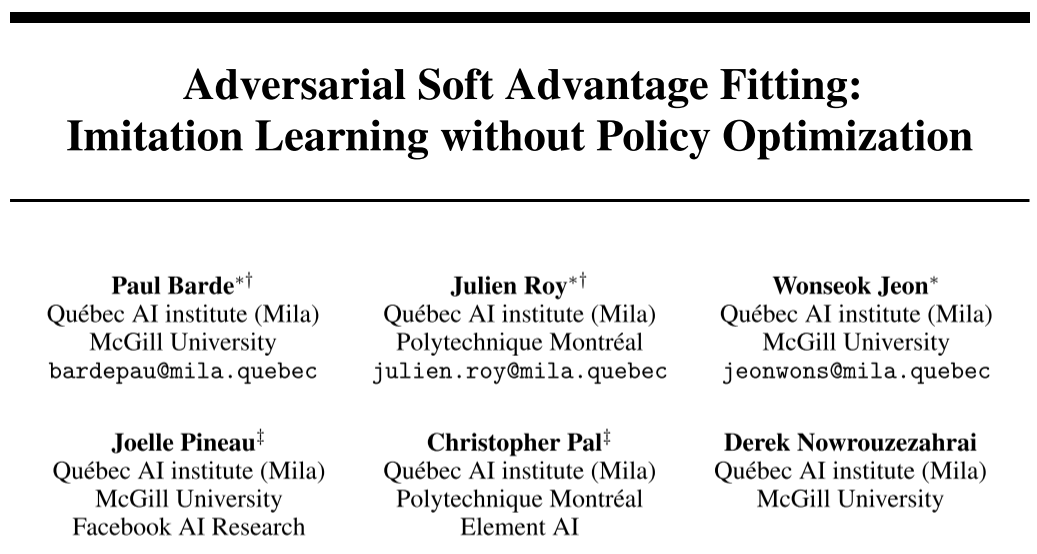
\includegraphics[width=0.6\linewidth]{paper_fig/info.png}
    \end{figure}
    \textit{Barde P, Roy J, Jeon W, et al. Adversarial soft advantage fitting: Imitation learning without policy optimization[C]. Advances in Neural Information Processing Systems, 2020, 33: 12334-12344.}
\end{frame}

% TOC
\begin{frame}{Table of Contents}
    \tableofcontents
\end{frame}

%%%%%%%%%%%%%%%%% Preliminaries %%%%%%%%%%%%%%%%
\section{Preliminaries}

\begin{frame}[allowframebreaks,fragile]{Preliminaries}
	\begin{itemize}
		\item Consider a $T$-horizon $\gamma$-discounted MDP $\mathcal{M} = \left \langle \mathcal{S}, \mathcal{A}, \mathcal{P}, \mathcal{P}_0, \gamma, r, T \right \rangle$, where
		      \begin{itemize}
			      \item $\mathcal{S}$ is the state space;
			      \item $\mathcal{A}$ is the action space;
			      \item $\mathcal{P}(s'|s,a) \in [0, 1]$ is the transition dynamics;
			      \item $\mathcal{P}_0(s_0)$ is the initial state distribution;
			      \item $\gamma \in [0,1]$ is the discount factor;
			      \item $r(s,a) \in \mathbb{R}$ with $r$ being bounded is the reward function;
			      \item $T \in \mathbb{N} \cup \{\infty\}$ is the horizon length.
		      \end{itemize}
		      We suppose that $\mathcal{S}$ and $\mathcal{A}$ are both finite, and $T<\infty$ for $\gamma = 1$.
		\item For any trajectory $\tau = (s_0, a_0, s_1, a_1, \ldots, s_{T-1}, a_{T-1}, s_T)$, define its probability $P_\pi(\tau)$ of being sampled on $\mathcal{M}$ as
		      \[
			      P_\pi(\tau) \triangleq \mathcal{P}_0(s_0)\prod_{t=0}^{T-1}\pi(a_t|s_t)\mathcal{P}(s_{t+1}| s_t, a_t).
		      \]
		\item For any policy $\pi$, we define its occupancy measure $\rho^\pi: \mathcal{S} \times \mathcal{A} \to [0, 1]$ as
		      \[
			      \rho^\pi(s, a) 
				  = \frac{1}{Z(\gamma, T)}\sum_{t=0}^{T-1} \gamma^t \pqty{\sum_{\tau:(s_t,a_t) = (s,a)} P_\pi(\tau)}
				  = \frac{1}{Z(\gamma, T)}\sum_{t=0}^{T-1} \gamma^t \Pr(s_t=s)\pi(a|s),
		      \]
		      where $Z(\gamma, T) = \sum_t^{T-1}\gamma^t$.
		\item The expected sum of discounted rewards can be expressed in term of the occupancy measure as
		      \[
			      J_\pi[r(s,a)] \triangleq \mathbb{E}_{\tau \sim P_\pi}\left[\sum_{t=0}^{T-1}\gamma^t r(s_t, a_t)\right] = Z(\gamma, T)\mathbb{E}_{(s, a) \sim \rho^\pi}[r(s,a)].
		      \]
		% \item Denote the imitator policy as $\pi$, the expert policy as $\pi_E$. We have the following objective of {\bf maximum entropy IRL}.
		%       \[
		% 	      \min_{r\in\mathcal{R}}\left(\max_\pi J_\pi[r + \mathcal{H}(\pi(\cdot|s))]\right) - J_{\pi_E}[r],
		%       \]
		%       where $\mathcal{H}(\pi(\cdot|s)) = \mathbb{E}_{a\sim\pi(\cdot|s)}[-\log(\pi(a|s))]$.
		\item By properly regularizing the learned reward function $r$, \citep{gail} associated the maximum entropy IRL problem with GAN, thus getting GAIL's objective:
		      \[
			      \min_\pi \max_D \mathbb{E}_{(s,a)\sim \rho^{\pi_E}}\left[\log\left(D(s,a)\right)\right] + \mathbb{E}_{(s,a)\sim \rho^{\pi}}\left[\log\left(1-D(s,a)\right)\right],
		      \]
		      which is equivalent to the following Jensen-Shannon divergence minimization problem,
		      \[
			      \min_\pi D_\text{JS}(\rho_\pi, \rho_{\pi_E}).
		      \]
			  %  J_\pi[\mathcal{H}(\pi(\cdot|s))]
	\end{itemize}
\end{frame}

%%%%%%%%%%%%%%%%% Motivation %%%%%%%%%%%%%%%%
\section{Motivation}

\begin{frame}{Motivation}
	\begin{itemize}
		\item GAIL performs not well in practice.
		      \begin{enumerate}
			      \item The min-max optimization procedure of GAIL is brittle and unstable;
			      \item The RL process is sample-inefficient and tricky.
		      \end{enumerate}
		\item {\color{red} Can we instead imitate the expert without adversarial training and RL policy optimization?}
	\end{itemize}
\end{frame}

%%%%%%%%%%%%%%%%% Method %%%%%%%%%%%%%%%%
\section{Method}

\begin{frame}[allowframebreaks,fragile]{Method}
	Consider the following new objective
	\begin{equation}\label{equ:1}
		\min_{\pi_G}\max_{\tilde{\pi}} L(\tilde{\pi}, \pi_G) := \mathbb{E}_{\tau\sim P_{\pi_E}}\left[\log D_{\tilde{\pi}, \pi_G}(\tau)\right] + \mathbb{E}_{\tau\sim P_{\pi_G}}\left[\log (1-D_{\tilde{\pi}, \pi_G}(\tau))\right],
	\end{equation}
	with the \textit{structured discriminator}:
	\[
		D_{\tilde{\pi}, \pi_G}(x) = \frac{P_{\tilde{\pi}}(\tau)}{P_{\tilde{\pi}}(\tau) + P_{\pi_G}(\tau)} = \frac{q_{\tilde{\pi}}(\tau)}{q_{\tilde{\pi}}(\tau) + q_{\pi_G}(\tau)}.
	\]
	Here $q_\pi(\tau)=\prod_{t=0}^{T-1}\pi(a_t|s_t)$.
	\begin{lemma}\label{lem:corp}
		For any stationary policy $\pi$, there is an one-to-one correspondence between $\pi$ and $q_\pi$ on $\mathcal{M}$.
	\end{lemma}
	\begin{proof}
		For any trajectory $\tau = (s_0, a_0, s_1, a_1, \ldots, s_{T-1}, a_{T-1}, s_T)$, we have that $P_\pi(\tau) = q_\pi \times \xi(\tau)$, with
		\[\xi(\tau) := \mathcal{P}_0(s_0)\prod_{t=0}^{T-1}\mathcal{P}(s_{t+1}|s_t, a_t).\]
		Since $\xi(\tau)$ is solely determined by the MDP $\mathcal{M}$, there is an one-to-one correspondence between $q_\pi$ and $P_\pi$. And from the definition of $\rho^\pi$, we know that $\rho^\pi$ can be computed directly from $P_\pi$. From Theorem 2 of \citep{syed2008apprenticeship}, we know that $\rho^\pi$ and $\pi$ is one-to-one corresponded. Thus concluding the proof.
	\end{proof}
	\begin{theorem}\label{thm:asaf}
		The optimal $\tilde{\pi}^* = \argmax_{\tilde{\pi}}L(\tilde{\pi}, \pi_G)$ for any $\pi_G$ in $\myeqref{equ:1}$ is such that $q_{\tilde{\pi}^*} = q_{\pi_E}$, and using $\tilde{\pi}^*$ as the generator policy $\tilde{\pi}^*$ minimizes $L(\tilde{\pi}^*, \pi_G)$, i.e,
		\[\tilde{\pi}^* \in \argmin_{\pi_G}\max_{\tilde{\pi}}L(\tilde{\pi}, \pi_G)=\argmin_{\pi_G}L(\tilde{\pi}^*, \pi_G).\]
	\end{theorem}
	\begin{proof}
		Theorem \ref{thm:asaf} states that given $L(\tilde{\pi}, \pi_G)$ defined in \myeqref{equ:1}:
		\begin{enumerate}[(a)]
			\item $\tilde{\pi}^* = \argmax_{\tilde{\pi}} L(\tilde{\pi}, \pi_G)$ satisfies $q_{\tilde{\pi}^*} = q_{\pi_E}$;
			\item $\pi^*_G = \tilde{\pi}^* \in \argmin_{\pi_G} L(\tilde{\pi}^*, \pi_G)$.
		\end{enumerate}
		We will give the corresponding proofs of (a) and (b) below.
		\begin{enumerate}[(a)]
			\item By expanding \myeqref{equ:1}, we have that
			      \[
				      \begin{aligned}
					      \argmax_{\tilde{\pi}} L(\tilde{\pi}, \pi_G)
					       & = \argmax_{\tilde{\pi}} \sum_{\tau_i} P_{\pi_E}(\tau_i)\log D_{\tilde{\pi}, \pi_G}(\tau_i) + P_{\pi_G}(\tau_i)\log(1-D_{\tilde{\pi}, \pi_G}(\tau_i))                         \\
					       & = \argmax_{\tilde{\pi}} \sum_{\tau_i} \xi(\tau_i)\left(q_{\pi_E}(\tau_i)\log D_{\tilde{\pi}, \pi_G}(\tau_i) + q_{\pi_G}(\tau_i)\log(1-D_{\tilde{\pi}, \pi_G}(\tau_i))\right) \\
					       & = \argmax_{\tilde{\pi}} \sum_{\tau_i} L_i(\tau_i).
				      \end{aligned}
			      \]
			      From Proposition 1 of \citep{gan}, we get
			      \[
				      D_{\tilde{\pi}, \pi_G}^* = \argmax_{D_{\tilde{\pi}, \pi_G}}L_i(\tau_i) = \frac{q_{\pi_E}(\tau_i)}{q_{\pi_E}(\tau_i) + q_{\pi_G}(\tau_i)}.
			      \]
			      Thus from the definition and monotonicity of $D_{\tilde{\pi}, \pi_G}^*$, we get $q_{\tilde{\pi}^*} = q_{\pi_E}$. Then by using Lemma \ref{lem:corp}, we conclude that $\tilde{\pi}^* = \pi_E$.
			\item we use the conclusion from (a), and get
			      \[
				      \begin{aligned}
					      \pi_G^*
					       & = \argmin_{\pi_G} L(\tilde{\pi}^*, \pi_G)                                                                                                                                                                                                 \\
					       & = \argmin_{\pi_G} \mathbb{E}_{\tau\sim P_{\pi_E}}\left[\log \frac{P_{\pi_E}(\tau)}{P_{\pi_E}(\tau) + P_{\pi_G}(\tau)}\right] + \mathbb{E}_{\tau\sim P_{\pi_G}}\left[\log \frac{P_{\pi_G}(\tau)}{P_{\pi_E}(\tau) + P_{\pi_G}(\tau)}\right] \\
					       & = \argmin_{\pi_G}-\log 4 + 2D_\text{JS}(P_{\pi_E}\|P_{\pi_G})                                                                                                                                                                             \\
					       & = \pi_E.
				      \end{aligned}
			      \]
			      Conclude the proof.
		\end{enumerate}
	\end{proof}
	From Theorem \ref{thm:asaf}, we find that optimizing the inner $\tilde{\pi}$ will give us the optimal outer $\pi_G$. We thus get ASAF, a new imitation learning algorithm with pseudocode shown in Algorithm \ref{algo:asaf}.

	\begin{algorithm}[H]
		% \KwOut{output result}
		% \KwResult{Write here the result }
		\caption{ASAF}
		\label{algo:asaf}
		\KwIn{expert trajectories $\mathcal{D}_E = \{\tau_i^{(E)}\}_{i=1}^{N_E}$}
			randomly initialize $\tilde{\pi}$ and set $\pi_G \gets \tilde{\pi}$\;
			\For{steps $m=0$ to $M$}{
				Collect trajectories $\mathcal{D}_G = \{\tau_i^{(G)}\}^{N_G}_{i=1}$ using $\pi_G$ \;
				\tcp{ASAF Update}
				Update $\tilde{\pi}$ by minimizing \myeqref{equ:2} \;
			 	$\pi_G \gets \tilde{\pi}$
			}
	\end{algorithm}

	\begin{equation}\label{equ:2}
		\mathcal{L}_{BCE}(\mathcal{D}_E,\mathcal{D}_G, \tilde{\pi}) \approxeq -\frac{1}{n_E}\sum_{i=1}^{n_E}\log D_{\tilde{\pi}, \pi_G}(\tau_i^{(E)})-\frac{1}{n_G}\sum_{i=1}^{n_G}\log\left(1- D_{\tilde{\pi}, \pi_G}(\tau_i^{(G)})\right),
	\end{equation}
	where $\tau_i^{(E)} \sim \mathcal{D}_E$, $\tau_i^{(G)} \sim \mathcal{D}_G$ and
	\begin{equation}\label{equ:emp_d}
		D_{\tilde{\pi}, \pi_G}(\tau) = \frac{\prod_{i=1}^{T-1}\tilde{\pi}(a_t|s_t)}{\prod_{i=1}^{T-1}\tilde{\pi}(a_t|s_t) + \prod_{i=1}^{T-1}\pi_G(a_t|s_t)}.
	\end{equation}

    \begin{remark}
		ASAF uses the full-length trajectory, which may be sample-inefficient. The authors also considered using a window size of $w$ or even transition-wise variants, and named them ASAF-$w$ and ASAF-1, respectively.
	\end{remark}
\end{frame}

%%%%%%%%%%%%%%%%% Experiments %%%%%%%%%%%%%%%%
\section{Experiments}

\begin{frame}[allowframebreaks,fragile]{Experiments}
	\begin{figure}
        \centering
        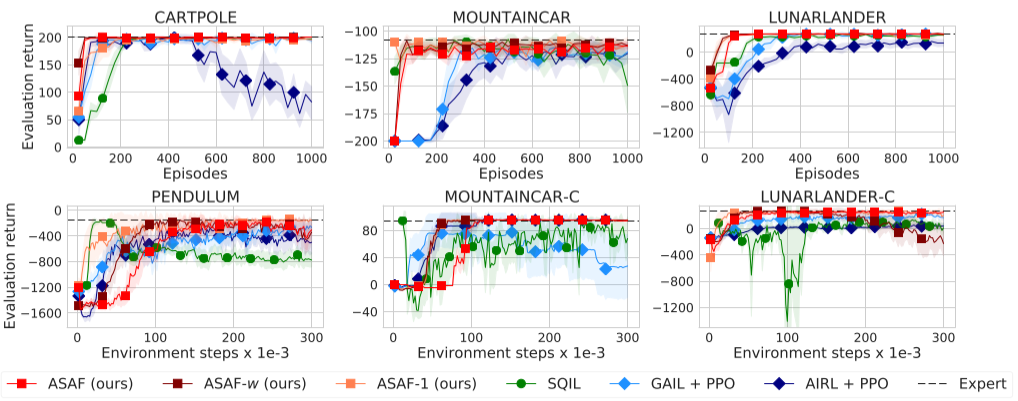
\includegraphics[width=0.8\linewidth]{paper_fig/exp_atari.png}
        \caption{Results on classic control and Box2D tasks for 10 expert demonstrations. First row contains discrete actions environments, second row corresponds to continuous control.}
    \end{figure}

    \begin{figure}
        \centering
        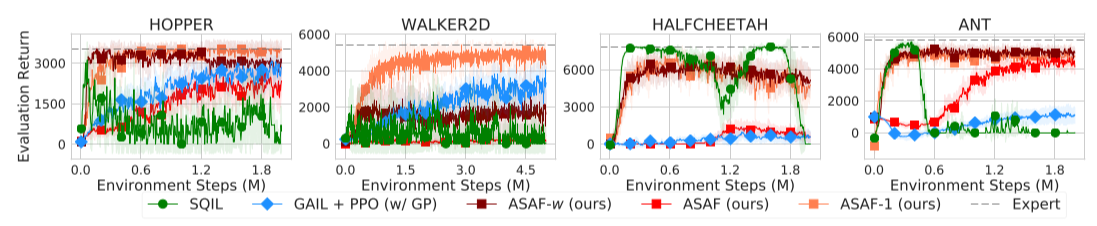
\includegraphics[width=0.8\linewidth]{paper_fig/exp_mujoco.png}
        \caption{Results on MuJoCo tasks for 25 expert demonstrations.}
    \end{figure}

\end{frame}

%%%%%%%%%%%%%%%%% Discussion %%%%%%%%%%%%%%%%
\section{Discussion}

\begin{frame}{Discussion}
	\begin{itemize}
		\item Model learning
		\[
			D_{\tilde{\mathcal{P}}, \mathcal{P}_G}(\tau) = \frac{\tilde{\mathcal{P}}(s_0)\prod_{i=1}^{T-1}\tilde{\mathcal{P}}(a_t|s_t)}{\prod_{i=1}^{T-1}\tilde{\mathcal{P}}(a_t|s_t) + \prod_{i=1}^{T-1}\mathcal{P}_G(a_t|s_t)}.
		\]
		\item Reduction to transition-wise scenario: The author also discussed a novel transition-wise objective (connected to \citep{DBLP:journals/corr/abs-1710-11248}), which is only suit for discrete action space.
		% \begin{itemize}
		% 	\item Directly reduce \myeqref{equ:emp_d} into a transition-wise objective;
		% 	\[
		% 		D_{\tilde{\pi}, \pi_G}(s,a) = \frac{\tilde{\pi}}{\tilde{\pi}+\pi_G},
		% 	\]
		% 	$\Longrightarrow$ $\tilde{\pi}^* = \commentedbox{\frac{d^{\pi_E}(s)}{d^{\pi_G}(s)}}{\tiny We need other tools to estimate it} \times \pi_E \neq \pi_E$.
		% 	\item The author also discussed a novel transition-wise objective (connected to \citep{DBLP:journals/corr/abs-1710-11248}), which is suit for discrete action space.
		% \end{itemize}
		\item We can use any policy to sample fake trajectories.
	\end{itemize}
\end{frame}

\begin{frame}{The End}
    \begin{center}
        {\huge Thanks!} \\
        \vspace{0.3cm}
        {\huge Q \& A}
    \end{center}
\end{frame}

%%%%%%%%%%%%%%%%% References %%%%%%%%%%%%%%%%
\begin{frame}{References}
	\setcitestyle{authoryear,round,citesep={;},aysep={,},yysep={;}, sort}
	\setcitestyle{numbers}
	\bibliographystyle{reference}
	\bibliography{reference}
\end{frame}

\end{document}